\documentclass{jarticle}
\usepackage{robomech2022}
\usepackage[dvipdfmx]{graphicx}
\usepackage{subcaption}
\captionsetup[figure]{justification=centering}
\captionsetup[table]{justification=centering}

\begin{document}
\makeatletter
\title{視覚と行動のend-to-end学習により経路追従行動をオンラインで\\模倣する手法の提案}
{―経路への復帰行動の解析と復帰行動を強化する教師データ収集法の検討―}
{A proposal for an online imitation method of
path-tracking behavior by end-to-end\\ learning of vision and action}
{-Analysis of return-to-pathway behavior and
a method of collecting training data to
enhance\\ return-to-pathway behavior-}

\author{
\centering
\begin{tabular}{ccc}
 \hspace{1zw}○学\hspace{1zw}今井悠月 (千葉工大)&\hspace{2zw}\hspace{1zw} 清岡優祐(千葉工大)&\hspace{1zw}学\hspace{1zw} 春山健太(千葉工大)\\
 \hspace{1zw}\hspace{1zw}正\hspace{1zw}上田隆一 (千葉工大)&\hspace{1zw}正\hspace{1zw} 林原靖男(千葉工大)\\

 &\\
 \multicolumn{3}{c}{\small Yuzuki IMAI, Chiba Institute of Technology, s20c1015as@s.chibakoudai.jp}\\
 \multicolumn{3}{l}{\hspace*{15.6mm}\small Yusuke KIYOOKA, Kenta HARUYAMA, }\\
 \multicolumn{3}{l}{\hspace*{15.8mm}\small Ryuichi UEDA and Yasuo HAYASHIBARA, Chiba Institute of Technology}\\
\end{tabular}
}
\makeatother

\abstract{ \small 
We have proposed an online imitation method of path-tracking behavior based on end-to-end learning of vision and action.
In recent years, many studies of autonomous movement using end-to-end learning have been reported, but these studies have also observed deviations from the target path.
One of the possible reasons for this is the lack of training data for returning to the path.
In this paper, we perform end-to-end learning to follow a route generated by a map-based navigation system. The dataset was collected in two ways, one is to learn only the area around the route and the other is to learn the state away from the route, and the generated path-tracking behaviors were analyzed.
In addition, we proposed a new method of collecting teacher data to reinforce the behavior of returning to the path, and verified the effectiveness of the method by experiments using a simulator.
}

\date{} 
\keywords{autonomous movement, navigation, end-to-end learning, dataset}

\maketitle
\thispagestyle{empty}
\pagestyle{empty}

\small

\section{緒言}
% 我々は, 入出力関係を直接学習する end-to-end 学習器により,
% 人の操作ではなく, 地図ベースのナビゲーションシステムを用いた
% 経路追従行動を視覚に基づいてオンラインで模倣する手法を提案し,
% その有効性を実験により検証してきた[1][2].
我々は, 従来から経路追従行動を視覚に基づきオンラインで模倣する手法を提案してきた.[1][2].
模倣には, 入出力関係を直接学習する end-to-end 学習器を用いる.
これにより, 地図ベースのナビゲーションシステムを画像の入力のみで実現できることが期待される.
地図ベースのナビゲーションでは, LiDAR や IMU, ホイールオドメトリなど複数のセンサを用いて
占有格子地図を作成する.
その地図を用いて自己位置推定, 経路計画, 制御などの複数のタスクを実行する.
これらによって, 目的の場所へ自律的に移動する手法である[3].
近年, このような画像を入力とした end-to-end 学習による自律移動手法が研究されている.
例えば, Muller らは, 人が操作したコントローラ操作を教師データとして学習することで, 
オフロード環境で障害物を回避しながら走行できることを確認した[4].
また, Bojarski らは画像と人が操作した制御コマンドを end-to-end 学習するこ
とで, 自動車を対象とした自律移動手法を提案した[5].
しかし, それらの研究では必ずしも学習した経路を追従できる
わけではなく, 目標とする経路から外れていく様子が確認されている.
その一因として, 目標経路へ復帰するための学習データが不足していることが考えられる.

そこで本稿では, カメラ画像を入力とした end-to-end 学習による自律移動手法において,
常に経路周辺を学習する場合と, 目標経路周辺だけでなく目標経路から離れた状態も学習する場合の
二つの方法でデータセットを収集し, 学習を行う[6]. そして, その学習によって生成された経路追従行動の解析
を行い, 離れた状態からの復帰行動を学習することが, 有効であるかを明らかにする. それに加え, 
目標経路への復帰行動を強化する教師データ収集法を新たに提案し, 有効性を検証することを目的とする.

 
\section{地図ベースのナビゲーションを模倣する手法}
地図ベースのナビゲーションをオンラインで模倣する手法を示す.
本手法は, 地図ベースのナビゲーションシステムの出力である角速度を教師データとして学習し, 
画像を入力とした学習器の出力によってロボットを制御する. 
手法は学習器の訓練を行う学習フェーズと, 訓練結果を検証するテストフェーズに分かれる.

\subsection{学習フェーズ}
図1に学習フェーズのシステムを示す. 学習フェーズでは,ロボットはROSのナビゲーションパッケージである
navigation[7]を用いて自律移動を行う. それと同時に, 画像とnavigationから出力される目標角速度を
ペアにしたデータセットを収集し, end-to-end 学習を行う.
地図ベースのナビゲーションは LiDAR とオドメトリを入力とするのに対し, 学習器は画像
を入力とする. 本手法を用いて学習することで, LiDAR, オドメトリを使用した時と同じ行
動を, 画像のみで行うことが期待される. 


\begin{figure}[h!]
  \centering
   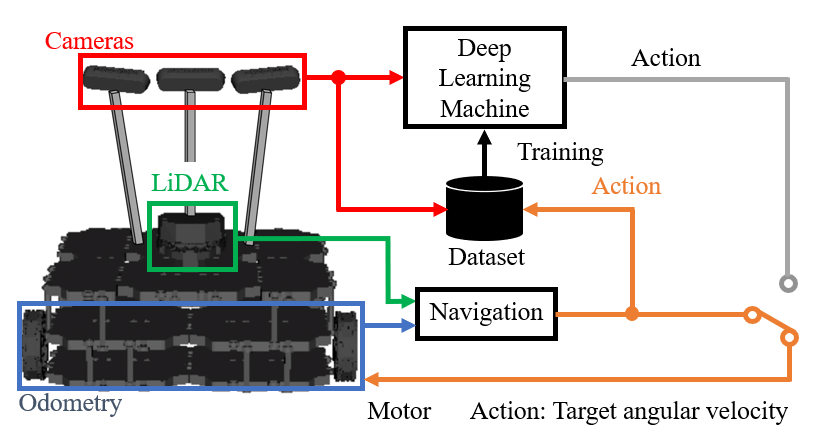
\includegraphics[height=42mm]{./figs/ga.png}
   \caption{Learning phase}
\end{figure}


\subsection{テストフェーズ}
テストフェーズでは, 図2のように学習フェーズで学習したモデルを用いてロボット
を制御し, 自律移動できるかテストする. 64 x 48 にリサイズした画像を学習器に入力し, その
出力をロボットの目標角速度としてロボットを自律移動させる.
ロボットの角速度は学習器の出力を用いるが, 並進速度は学習フェーズと同様に一定(0.2m/s)とする.
なお, テストフェーズでは3台のカメラのうち, 中央のカメラのみ使用する.

\begin{figure}[h!]
  \centering
   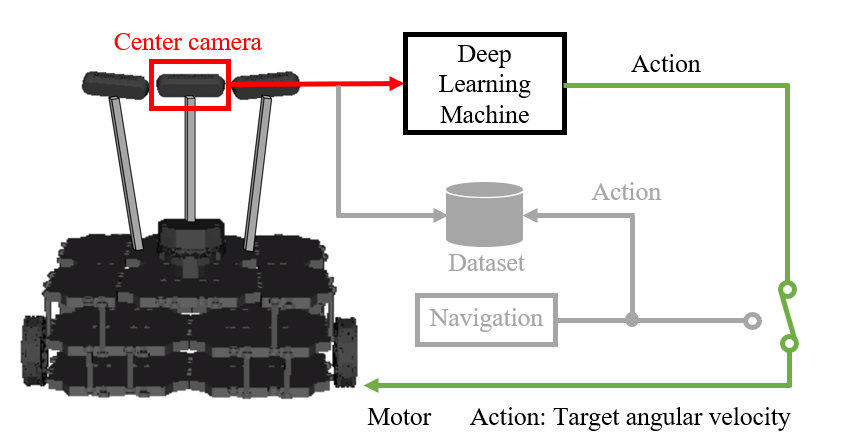
\includegraphics[height=42mm]{./figs/te.png}
   \caption{Test phase}
\end{figure}



\subsection{学習器について}
ネットワークの構成と学習方法について述べる.本研究は,
画像を入力,角速度を出力として end-to-end 学習を行う.
ネットワークは, 図3に示すように, 入力層 1 ,畳み込み層 3 ,全結合層 2 ,出力層 1 の全 7 層で構成されている.
また学習をする際, 1 ステップに付きデータセットの中からランダムに 8 個のデータを抽出し, 
その8 個のデータで学習を行っている.


\begin{figure}[h!]
  \centering
   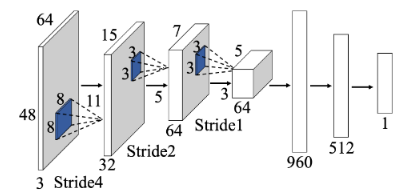
\includegraphics[height=30mm]{./figs/gaku2.png}
   \caption{Structure of the network}
\end{figure}


\section{地図ベースのナビゲーションを模倣する実験}

経路周辺だけでなく,経路から離れた状態を学習することが経路追従行動を模倣
する上で有効であることを明らかにするためにシミュレータを用いた実験を行う. 
実験は, 経路周辺を学習した場合と, 経路から離れた状態も学習する場合の二つのデータセット収集
方法で行い, 学習器の出力で経路を追従できるか調査する.

\subsection{実験装置}
実験にはシミュレータ[8]を用いた.
環境は図4に示すような, 千葉工業大学津田沼キャンパス2号館3階を模したモデルである.
ロボットは,  Turtlebot3[9] にカメラを 3 つ取り付けたモデルを用いた. 
図5にロボットが追従する経路を示す.ロボットはこの図の赤い線を追従するように学習を行う.

\begin{figure}[htbp]
  \begin{minipage}{0.5\hsize}
   \centering
   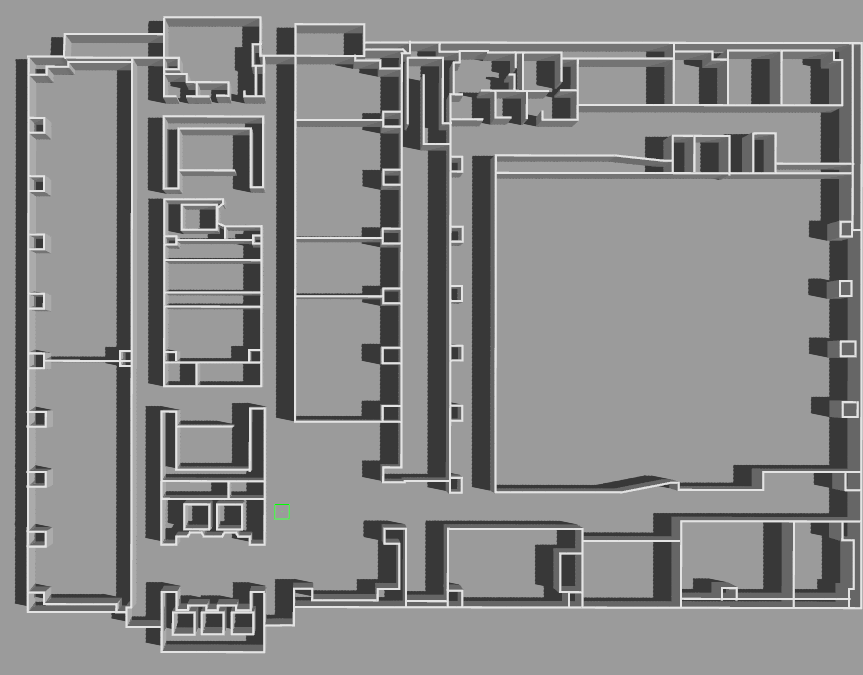
\includegraphics[width=40.1mm]{figs/gazebo.png}
   \caption{Experiment model}
  \end{minipage}
  \begin{minipage}{0.5\hsize}
   \centering
   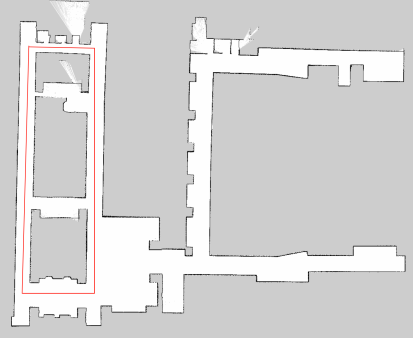
\includegraphics[width=38.5mm]{figs/rviz.png}
   \caption{Target path}
  \end{minipage}
 \end{figure}


\subsection{比較するデータセット収集方法}
比較する 2 つのデータセットの収集方法を述べる.\\

\subsubsection{経路周辺の状態のみを学習する手法}
経路周辺の状態のみを学習する手法を図6に示す.ロボットは常に navigation の出力
で経路を追従するように行動する.そして, その行動を常にデータセットとして収集する.
本稿では, このデータセット収集方法を Path following method と呼ぶ.

\begin{figure}[h!]
  \centering
   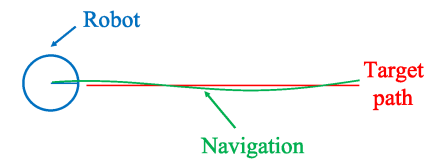
\includegraphics[height=30mm]{./figs/dl.png}
   \caption{Path following method}
\end{figure}

\subsubsection{経路から離れた状態も学習する手法}
経路から離れた状態も学習する手法を図7に示す.経路周辺と経路から離れたときで, 
ロボットを制御するモジュールを切り替えている.経路周辺では, 学習器の出力を用いている.
ロボットが経路から離れた場合,  navigation で経路へ復帰させる. データセットに追加
するデータは常に navigation の出力である.このように経路周辺で学習器の出力を用いてロ
ボットを制御することで,  Path following method に比べて, 経路から離れた状態のデータを
多く収集できることが期待できる.このデータセット収集方法を本稿では Using learning
machine output method と呼ぶ.

\begin{figure}[h!]
  \centering
   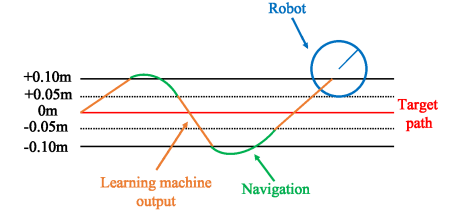
\includegraphics[height=42mm]{./figs/dl_use.png}
   \caption{Using learning machine output method}
\end{figure}

\subsection{実験方法}
実験は学習フェーズの後, テストフェーズに移行し, コースを1周できるかを確認する.
学習フェーズでは 2 章で説明した, 地図ベースのナビゲーションを模倣する手法を用いる.
データセットは 0.2 秒周期で取得し,  10000 エピソード学習行った.
壁に衝突することなくコースを1周することができれば経路追従に成功したと判断した. この
実験を二つのデータセット収集方法でそれぞれ 50 回ずつ行った.

\subsection{実験結果}
実験の結果を表1に示す. Path following method で学習したモデルでロボットを
制御した場合, 一度もコースを 1周することができなかった.それに対し, Using learning
machine output method では,  50 回中 29 回コースを1周することに成功した.

ここで, データセットに含まれる目標経路からの距離で分類した学習データの割合のグラフ
を図8に示す.これは, それぞれのデータセット収集方法で 50 回ずつ実験を行い, 平均
した結果である. Using learning machine output method の方が Path following method に
比べて目標経路から離れた状態のデータセットを多く収集している様子が見られる.
これらのことから, 目標経路から離れた状態のデータセットを多く収集することで経路を追
従できる確率が高まることが一例ではあるが確認された.

\begin{table}[htbp]
  \centering
  \caption{Number of successes} \vspace*{2mm}
    \scalebox{0.85}[0.85] {
    \begin{tabular}{|c|c|}
      \hline\hline
      Dataset collection method & Number of successes \\
      \hline\hline
      Path following method & 0/50 \\
      Using learning machine output method & 29/50 \\
      \hline
    \end{tabular} }
\end {table}


\begin{figure}[htbp]
  \centering
   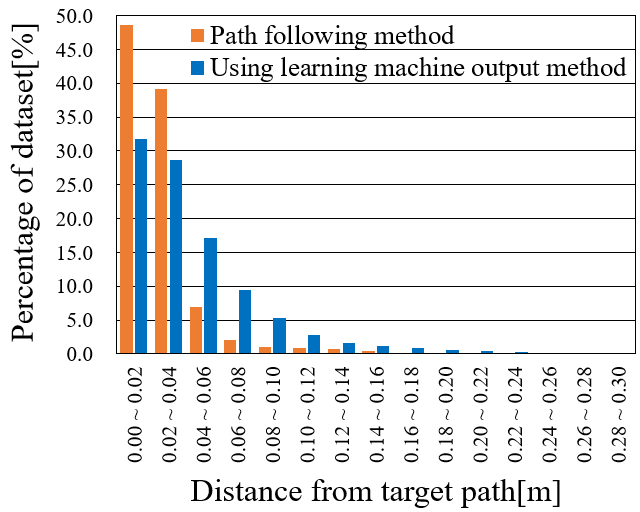
\includegraphics[height=55mm]{./figs/tes.png}
   \caption{Percentage of the dataset in the experiment}
\end{figure}


\section{生成された経路追従行動の解析}
\subsection{解析方法}
生成された経路追従行動を比較するため, 実験で生成した学習済みモデルでロボットを制御し, 
その経路追従行動を調査する.ロボットの初期位置を,  図9のような場所に指定してロボットを走行させる.
ロボットの進行方向を基準にして右側を正の値とし, 左側を負の値とした.調査する場所は, 曲がり角付近とした. 
この曲がり角というのは, 実験において, 経路追従行動に失敗する回数が特に多かった場所である.
この場所を対象に,  84 カ所からロボットを走行させ, 経路に戻ることができるのか調査した.
また, 一つの座標につき 5方向(目標経路を追従するように制御した時のロボットの向きを基準とし
て -10 度〜 10 度を± 5 度ずつ傾けた方向)をロボットの初期姿勢とした. 
つまり,  一つの学習済みモデルにつき 420 カ所の初期位置からロボットを走行させ, 
経路へ復帰できるのか調査した.ここで, 図10に示すように, 壁に衝突することなく目標経路に近づいて, 
経路周辺 (0.1m 以内)を 4秒間走行することができれば経路復帰に成功したと判断した.
逆に, 壁に衝突した場合を経路復帰に失敗したと判断した.


\begin{figure}[h!]
  \centering
   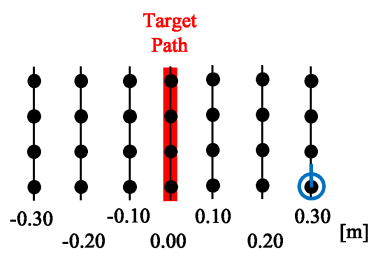
\includegraphics[height=36mm]{./figs/k.png}
   \caption{Initial position of the robot during analysis}
\end{figure}


\begin{figure}[htbp]
  \begin{minipage}[t]{0.5\linewidth}
    \centering
    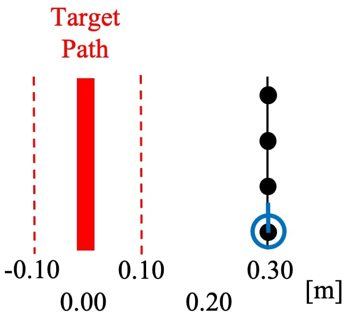
\includegraphics[keepaspectratio, scale=0.43]{figs/1.png}
    \subcaption{Initial position}
  \end{minipage}
  \begin{minipage}[t]{0.5\linewidth}
    \centering
    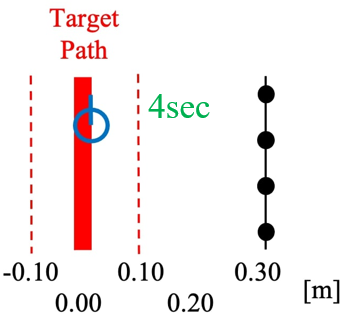
\includegraphics[keepaspectratio, scale=0.43]{figs/2.png}
    \subcaption{Conditions for success}
  \end{minipage}\vspace*{2mm}
\vspace*{-2.5mm}
  \begin{minipage}[t]{0.5\linewidth}
    \centering
    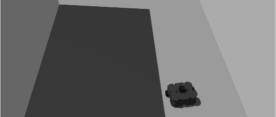
\includegraphics[keepaspectratio, scale=0.32]{figs/init4.png}
    \subcaption{Robot in initial position}
  \end{minipage}
  \begin{minipage}[t]{0.5\linewidth}
    \centering
    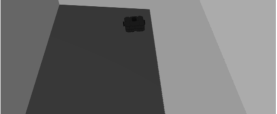
\includegraphics[keepaspectratio, scale=0.33]{figs/return3.png}
    \subcaption{Robot back near path}
  \end{minipage}\vspace*{4mm}
  \caption{Analysis of the path-tracking behavior}
\end{figure}


\subsection{解析結果}
解析の結果の一部を図11, 図12に示す. 図11は, ロボットが走行し始めた場
所と経路復帰に成功した回数を示している. 1 つの座標につきロボットの方向を変えながら
5回経路に戻れるか調査しており, 経路復帰に成功した回数を色で表している.
この結果から, Using learning machine output methodでは曲がり角に入る前で左にいると, 
経路復帰に失敗するおそれがあるが, それ以外は経路追従に成功する様子が見られる.
それに対して, Path following methodは左右に関係なく失敗している様子が見られる.
図12は経路復帰に失敗した時のロボットの軌跡を表している. 図12(a)に示すように,
Path following method では曲がり角で, 曲がることなく直進する傾向があったのに対し, 
図12(b)に示すように, Using learning machine output method では, 曲がり角で曲がる
動作がより多く確認できた.
また, 3章で示した実験で生成した 50 個の学習モデルのうち 5 個を解析し, その平均した
結果を, 図13に示す.この図は, 目標経路からの距離ごとに経路復帰に成功した割合を表している. 
Path following method では経路周辺が経路復帰できる確率が高いが, 経路から
離れると経路に復帰する確率は低くなっていく傾向が見られた.それに対し, Using learning
machine output method は, 進行方向を基準とした経路の右側からロボットを走行させた場
合, Path following method と比べて経路復帰できる確率が高いことが分かった.
結果的に, これらの解析から経路周辺の状態だけでなく経路から離れた状態も学習することで, 経路
から離れても経路復帰できる確率が高まることが確認された.

\begin{figure}[htbp]
  \begin{minipage}[t]{0.5\linewidth}
    \centering
    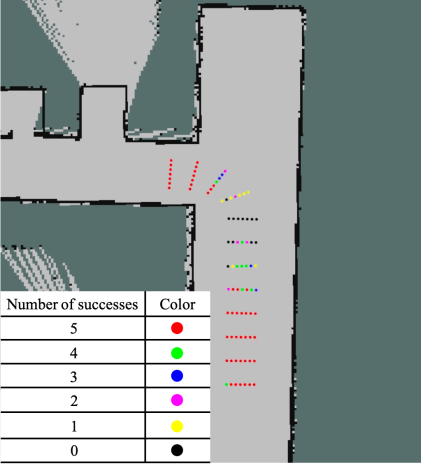
\includegraphics[keepaspectratio, scale=0.2]{figs/a.png}
    \subcaption{Path following method}
  \end{minipage}
  \begin{minipage}[t]{0.5\linewidth}
    \centering
    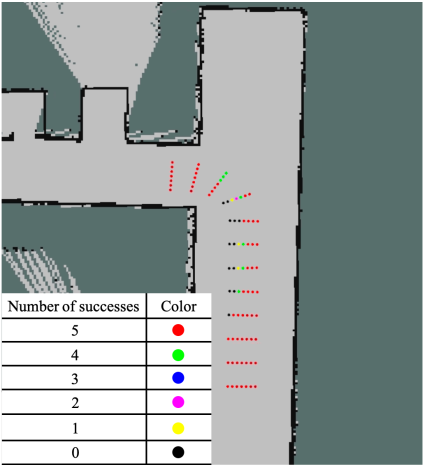
\includegraphics[keepaspectratio, scale=0.2]{figs/b.png}
    \subcaption{Using learning machine output method}
  \end{minipage}\vspace*{2mm}
  \caption{Number of return to path}
\end{figure}
\vspace*{-2.5mm}
\begin{figure}[htbp]
  \begin{minipage}[t]{0.5\linewidth}
    \centering
    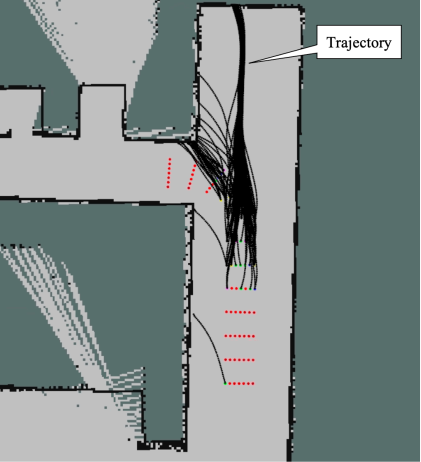
\includegraphics[keepaspectratio, scale=0.2]{figs/c.png}
    \subcaption{Path following method}
  \end{minipage}
  \begin{minipage}[t]{0.5\linewidth}
    \centering
    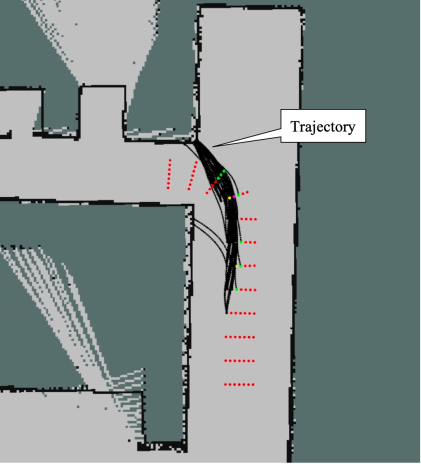
\includegraphics[keepaspectratio, scale=0.2]{figs/d.png}
    \subcaption{Using learning machine output method}
  \end{minipage}\vspace*{2mm}
  \caption{Trajectory of robot that failed to follow the path}
\end{figure}

\begin{figure}[h!]
  \centering
   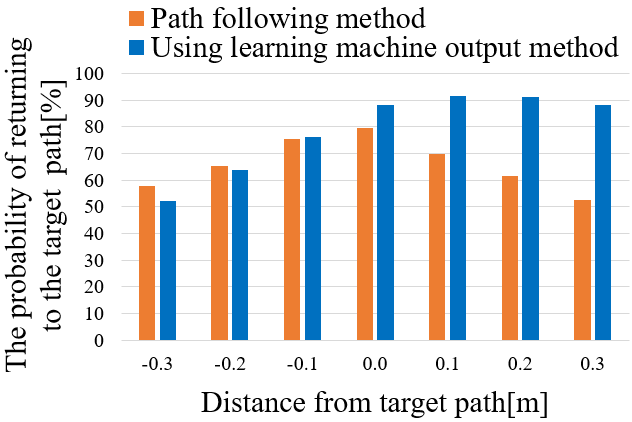
\includegraphics[height=38.97mm]{./figs/kaiseki2.png}
   \caption{Percentage able to return to the pathway}
\end{figure}



\section{経路復帰行動を強化する教師データ収集法の検討}

経路から離れた状態も学習することで, 経路を追従できる確
率が高まることが確認された. そのため, 本章では経路復帰行動を強化するためのデータセット収
集方法を提案し, 有効性を検証する.

\subsection{提案するデータセット収集法}
経路から離れた状態からの復帰行動をより多く学習する手法を提案する. 
具体的には, 経路からの距離が0.05m 未満であれば1つ, 
0.05m 以上0.10m 未満であれば2つ, 0.1m 以上であれば3つ同じデータをデータセットに加える.
本稿では, このデータセット収集法を Enhanced return action method と呼ぶ.

\begin{figure}[h!]\vspace*{-3mm}
  \centering
   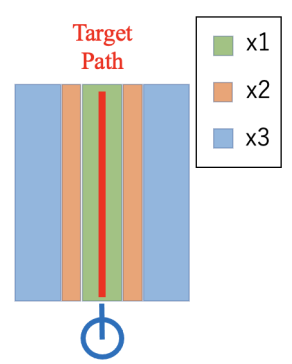
\includegraphics[height=45mm]{./figs/method.png}
   \caption{Enhanced return action method}
\end{figure}


\subsection{シミュレータを用いた実験}
提案するデータセット収集法の有効性を検証するため, シミュレータを用いた実験を行う.
実験装置と実験方法は3章と同様である.
\vspace*{2.5mm}
\subsubsection{実験結果}
実験の結果を表2に示す. 提案するデータセット収集法の方が経路を追従できる確率が高い様子が見られた.
ここで, データセットに含まれる目標経路からの距離と学習データの割合のグラフを
図15に示す. Enhanced return action method は, より経路から離れた状態のデータを多く収集している
ことが確認された.


\begin{table}[h!]
  \centering
  \caption{Number of successes} \vspace*{2mm}
    \scalebox{0.85}[0.85] {
    \begin{tabular}{|c|c|}
      \hline\hline
      Dataset collection method & Number of successes \\
      \hline\hline
      Using learning machine output method & 29/50 \\
      Enhanced return action method & 42/50\\
      \hline 
    \end{tabular} }
\end {table}


\begin{figure}[h!]\vspace*{-5mm}
  \centering
   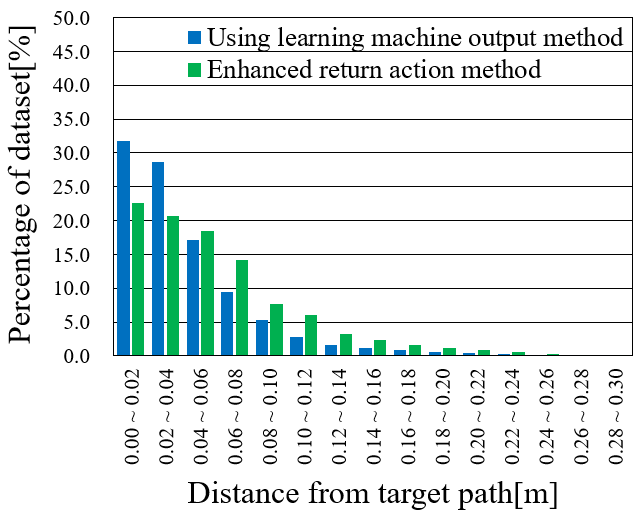
\includegraphics[height=55mm]{./figs/tes2.png}
   \caption{Percentage of the dataset in the experiment}
\end{figure}

\subsection{生成された経路追従行動の解析}
4 章で行った解析と同様に, 本章で提案する手法によって生成した経路追従行動を調査する.
5.2.3 章で示した実験で生成した 50 個の学習モデルのうち 5 個を解析し, その結果を平均し
たものを図16に示す. この図は, 目標経路からの距離ごとに経路復帰に成功した割合を表
している. この結果から, 目標経路の周辺全てにおいて, 提案する手法は,
Using learning machine output method と比べて経路復帰に成功する確率が高いことが確認
できた.

\begin{figure}[h!]\
  \centering
   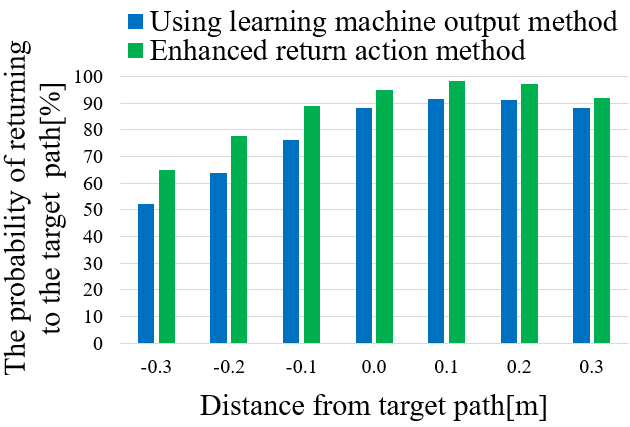
\includegraphics[height=40mm]{./figs/kaiseki2-2.png}
   \caption{Percentage able to return to the pathway}
\end{figure}


\section{結言}
本稿では, 従来から提案する経路追従行動を模倣する手法において, 目標経路から離れた
状態も学習することが経路復帰に有効であることを明らかにした.
その後, 経路復帰行動を強化するための教師データ収集方法を新たに提案し, シミュレータを用いた実験
により, 手法の有効性を一例ではあるが示した.
また, 学習済みモデルを用いて, 経路から離れた位置から経路に復帰できるかを解析し,
経路から離れた状態をより多く学習したほうが経路追従できる確率が高くなることを確認した.
\vspace*{4mm}

\footnotesize
\begin{thebibliography}{99}

\bibitem{1}
岡田眞也, 清岡優祐, 上田隆一, 林原靖男: “視覚と行動の end-
to-end 学習により経路追従行動 をオンラインで模倣する手法
の提案”, 計測自動制御学会 SI 部門講演会 SICE-SI2020 予稿
集, pp.1148-1152(2020).

\bibitem{2}
岡田眞也, 清岡優祐, 春山健太, 上田隆一, 林原靖男:“視覚と
行動の end-to-end 学習により経路追従行動 をオンラインで
模倣する手法の提案 -経路追従行動の修正のためにデータセッ
トを動的に追加する手法の検討-”, 計測自動制御学会 SI 部門
講演会 SICE-SI2021 予稿集, pp.1066-1080(2021).

\bibitem{3}
W. Schwarting, J. Alonso-Mora, and D. Rus.
Planning and decision making for
autonomous vehicles . Annu. Rev, Vol. 1, No. 1, pp. 188-210, May 2018.

\bibitem{4}
U. Muller, J. Ben, E. Cosatto, B. Flepp, and Y. Cun. ”Off-road obstacle avoidance
through end-to-end learning”. Advances in neural information processing systems,
Vol. 18, 2005.

\bibitem{5}
Bojarski, Mariusz, and et al.
”End to end learning for self-driving cars”.
arXiv:1604.08316, 2016.

\bibitem{6}
清岡優祐 , 岡田眞也 , 岩井一輝 , 上田隆一 , 林原靖男: “視覚と行動の end-
to-end 学習により経路追従行動 をオンラインで模倣する手法
の提案 -データセットと生成された
経路追従行動の解析-”. 計測自動 制御学会 SI 部門講演会 SICE-SI2021 予稿集, pp.1071-1075(2021).

\bibitem{7}
ros-planning, navigation リポジトリ ( 最終閲覧日 :2023年 2月6日 ). https://
github.com/ros-planning/navigation.

\bibitem{8}
Nathan Koenig and Andrew Howard. ”Design and use paradigms for gazebo, an
open-source multi-robot simulator”. In 2004 IEEE/RSJ International Conference
on Intelligent Robots and Systems (IROS)(IEEE Cat. No. 04CH37566), Vol. 3, pp.
2149-2154. IEEE, 2004.

\bibitem{9}
Erico Guizzo and Ackerman Evan. ”The Turtlebot3 Teacher [Resources Hands On]”.
IEEE Spectrum, Vol. 54, pp. 19-20, August 2017.

\end{thebibliography}

\normalsize
\end{document}
